Afin de faciliter l'implémentation et rendre le projet plus facilement compréhensible, des patrons de conception ont été implémentés.
Ces derniers seront explicités dans les parties \ref{sec:fabrique} à \ref{sec:strategie}.

\subsubsection{Création des départements} \label{sec:fabrique} %Fabrique

\begin{figure}[!h]
\centering
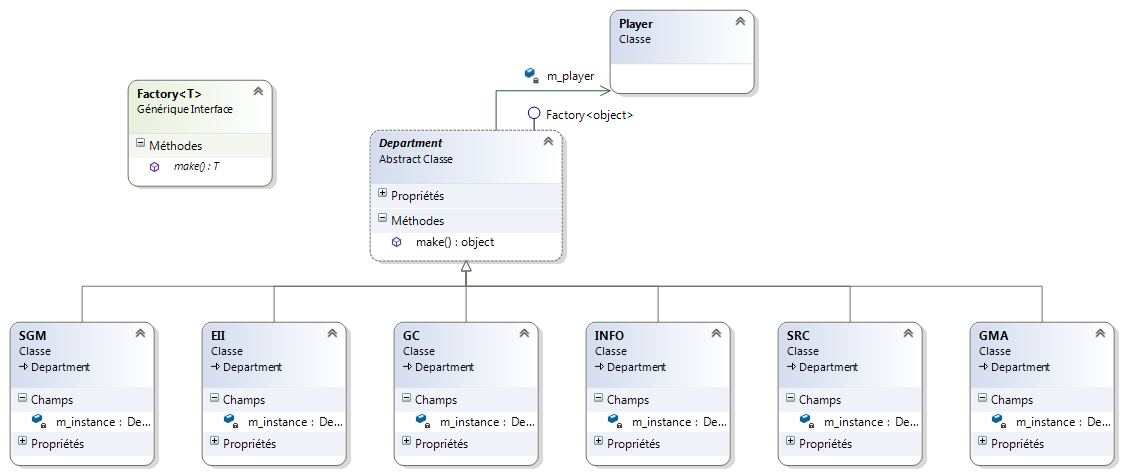
\includegraphics[width=\textwidth]{Parties/Images/UML_Dept.png}
\caption{Patron fabrique appliqué aux départements}
\label{fig:uml_dept}
\end{figure}

Le patron de conception \emph{fabrique} permet de créer des objets sans connaître leur classe, et éventuellement d'effectuer des opérations supplémentaires à la création.
Appliqué aux départements, elle permet à ces derniers de créer des unités qui leur sont spécifiques.
Par exemple, la méthode \emph{make()} du département \emph{INFO} ne créera pas les mêmes unités que celle du département \emph{EII}.
Son implémentation est détaillée dans la figure \ref{fig:uml_dept}.

\subsubsection{Création d'une partie} \label{sec:monteur} %Monteur

\begin{figure}[!h]
\centering
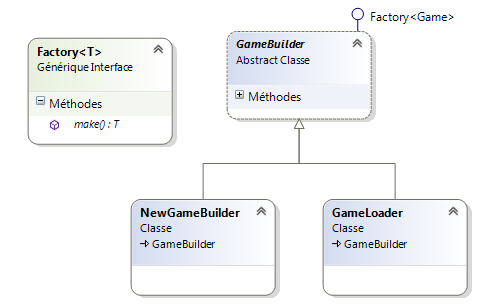
\includegraphics[width=0.7\textwidth]{Parties/Images/UML_Game.png}
\caption{Patron monteur appliqué à la création de parties}
\label{fig:uml_game}
\end{figure}

Le patron de conception \emph{monteur} permet de créer des objets suivant différents scénarios.
Ici, par exemple, on pourra créer une nouvelle partie ou charger une partie sauvegardée.
Son implémentation est détaillée dans la figure \ref{fig:uml_game}.

\subsubsection{Modélisation du terrain} \label{sec:poidsMouche} %Poids-mouche

\begin{figure}[!h]
\centering
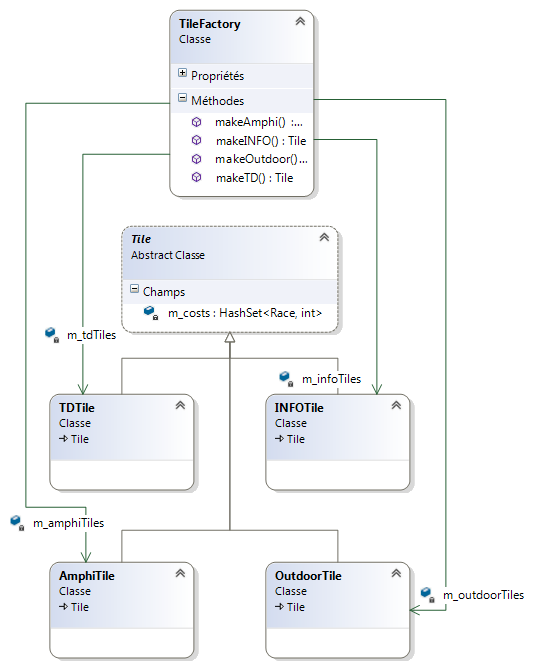
\includegraphics[width=0.6\textwidth]{Parties/Images/UML_Tiles.png}
\caption{Patron poids-mouche appliqué au terrain}
\label{fig:uml_tiles}
\end{figure}

Le patron de conception \emph{poinds-mouche} permet de contrôler le nombre d'instances d'un objet.
Dans le cas du terrain, chaque type de case (classes héritant de \emph{Tile}) ne sera instanciée qu'une fois.
Par exemple, les différentes salles informatiques pointeront vers la même instance de \emph{INFOTile}.
Son implémentation est détaillée dans la figure \ref{fig:uml_tiles}.

\subsubsection{Création de différents types de carte} \label{sec:strategie} %Stratégie

\begin{figure}[!h]
\centering
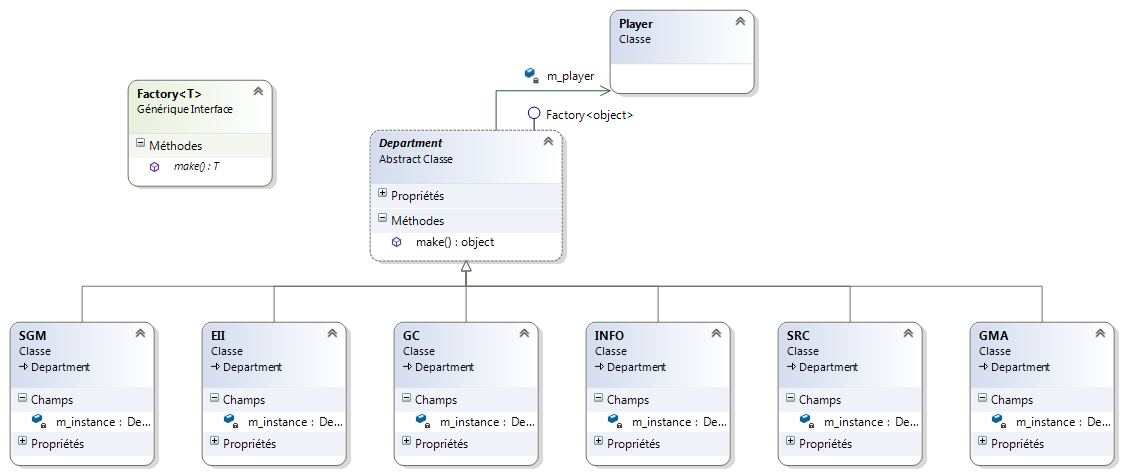
\includegraphics[width=\textwidth]{Parties/Images/UML_Dept.png}
\caption{Patron stratégie appliqué à la création des cartes}
\label{fig:uml_board}
\end{figure}

Le patron de conception \emph{stratégie} permet de réaliser une opération donnée de différentes manières.
Ici, il s'agit de créer différents types de cartes de différentes tailles.
Son implémentation est détaillée dans la figure \ref{fig:uml_board}.